\section{Experiments}

The experiments ask whether systems can update a concrete review issue after revision evidence, not merely whether they can produce plausible criticism.
We therefore read every result through two lenses: macro-F1 and per-label recovery under skew, and the failure modes in Table~\ref{tab:failure-taxonomy}.
The first two RQs quantify the accuracy trap; the latter two explain what breaks when models transfer across years.
Across all splits, three findings persist: (i) structured evidence gives the clearest in-domain gain, (ii) accuracy alone hides severe label-level failures, and (iii) prompted transfer remains brittle even with model voting and calibration rules.

\subsection{RQ1: Does Structure Help In Domain?}

\begin{table}[t]
\centering
\scriptsize
\setlength{\tabcolsep}{3pt}
\begin{tabular}{p{0.42\linewidth}rrr}
\toprule
Model & Accuracy & Macro-F1 & Fixed F1 \\
\midrule
Majority label & 0.581 & 0.184 & 0.000 \\
TF-IDF + LinearSVC & 0.561 & 0.376 & 0.510 \\
ModernBERT & 0.561 & 0.387 & 0.509 \\
MPNet & 0.581 & 0.389 & 0.554 \\
Structured without hard rules & 0.655 & 0.424 & 0.602 \\
Structured & \textbf{0.682} & \textbf{0.704} & \textbf{0.624} \\
\bottomrule
\end{tabular}
\caption{ICLR 2024 clean dev v7 results. Macro-F1 is the primary metric because label skew makes accuracy misleading.}
\label{tab:main-results}
\end{table}


Table~\ref{tab:main-results} shows that structured revision evidence substantially improves macro-F1 on ICLR 2024 clean dev v7.
The strongest semantic baseline, MPNet with a linear classifier, reaches 0.581 accuracy and 0.389 macro-F1.
The structured model reaches 0.682 accuracy and 0.704 macro-F1.
Removing structured hard overrides drops macro-F1 to 0.424, showing that explicit revision-follow-up cues drive much of the minority-label recovery.
This large drop also clarifies the model role: the strongest in-domain system is a diagnostic hybrid that combines learned scoring with benchmark-specific explicit cues.

\subsection{RQ2: When Does Accuracy Mislead?}

\begin{table}[t]
\centering
\scriptsize
\setlength{\tabcolsep}{3pt}
\begin{tabular}{p{0.18\linewidth}p{0.22\linewidth}rrr}
\toprule
Dataset & System & Accuracy & Macro-F1 & Fixed F1 \\
\midrule
ICLR 2024 & Majority & 0.581 & 0.184 & 0.000 \\
ICLR 2024 & TF-IDF & 0.561 & 0.376 & 0.510 \\
ICLR 2025 & Majority & 0.762 & 0.216 & 0.000 \\
ICLR 2025 & TF-IDF & 0.762 & 0.216 & 0.000 \\
\bottomrule
\end{tabular}
\caption{Null-baseline comparison. On the ICLR 2025 stress set, TF-IDF matches the majority baseline while failing fixed-case recovery.}
\label{tab:null-baselines}
\end{table}


Table~\ref{tab:null-baselines} shows why accuracy is insufficient.
On ICLR 2024, the majority-label baseline reaches the same accuracy as the best semantic baseline but has zero F1 for fixed, unresolved, and regressed cases.
On the ICLR 2025 repro stress set, TF-IDF exactly matches the majority baseline while assigning zero F1 to fixed cases.
This is the core evaluation failure RevTrack is designed to surface.

\subsection{RQ3: What Fails Qualitatively?}

The failure taxonomy is the bridge from aggregate scores to reviewer-facing risk and is a primary claim-bearing result, not an auxiliary error list.
It identifies five recurring modes.
\textit{Stale criticism} occurs when a model preserves an old concern after direct revision evidence fixes it.
\textit{Over-crediting} occurs when a long response acknowledges a limitation without resolving it.
\textit{Fixed under-recovery} occurs when the model keeps a resolved concern alive because the original critique remains lexically salient.
\textit{Partial-fix ambiguity} occurs when added evidence narrows but does not eliminate the concern.
\textit{Regression scarcity} remains a limitation: the current clean-dev pool contains only one regressed example, so regression performance is not yet a stable claim.
Table~\ref{tab:failure-taxonomy} turns these modes into paper-facing evidence rather than a post-hoc error list.
On expanded80, the structured transfer model over-credits unresolved concerns as fixed or partially fixed in 66 cases, TF-IDF misses all four fixed examples and all six regressed examples, and the strongest issue-ledger model still makes four partial/full-boundary errors.
These counts should be read as active-frontier diagnostics, not natural prevalence.

\begin{table}[t]
\centering
\scriptsize
\setlength{\tabcolsep}{3pt}
\begin{tabular}{p{0.22\linewidth}p{0.31\linewidth}p{0.35\linewidth}}
\toprule
Failure mode & Pattern & Evidence use \\
\midrule
Stale criticism & predicts partially\_fixed or unresolved because the original concern remains semantically plausible & This example separates revision-aware judgment from static semantic plausibility. \\
Over-crediting & over-credits unresolved concerns as fixed or partially fixed (66 expanded80 errors) & This is the practical stale-assistant failure: the model would stop tracking an unresolved concern. \\
Fixed under-recovery & keeps a fixed concern alive as partially fixed or unresolved (4 expanded80 errors) & This motivates fixed-case F1 rather than accuracy-only reporting. \\
Regression blindness & misses cases where the revision introduces or worsens a problem (6 expanded80 errors) & This justifies keeping the regressed label while avoiding strong regression-performance claims. \\
Partial/full boundary & collapses partial resolution into fixed (4 expanded80 errors) & This is the central label-boundary risk for benchmark reliability. \\
\bottomrule
\end{tabular}
\caption{Qualitative failure taxonomy used to interpret RevTrack errors. Expanded80 counts are from the user-confirmed standard active frontier and should not be read as natural prevalence.}
\label{tab:failure-taxonomy}
\end{table}


\begin{figure*}[t]
\centering
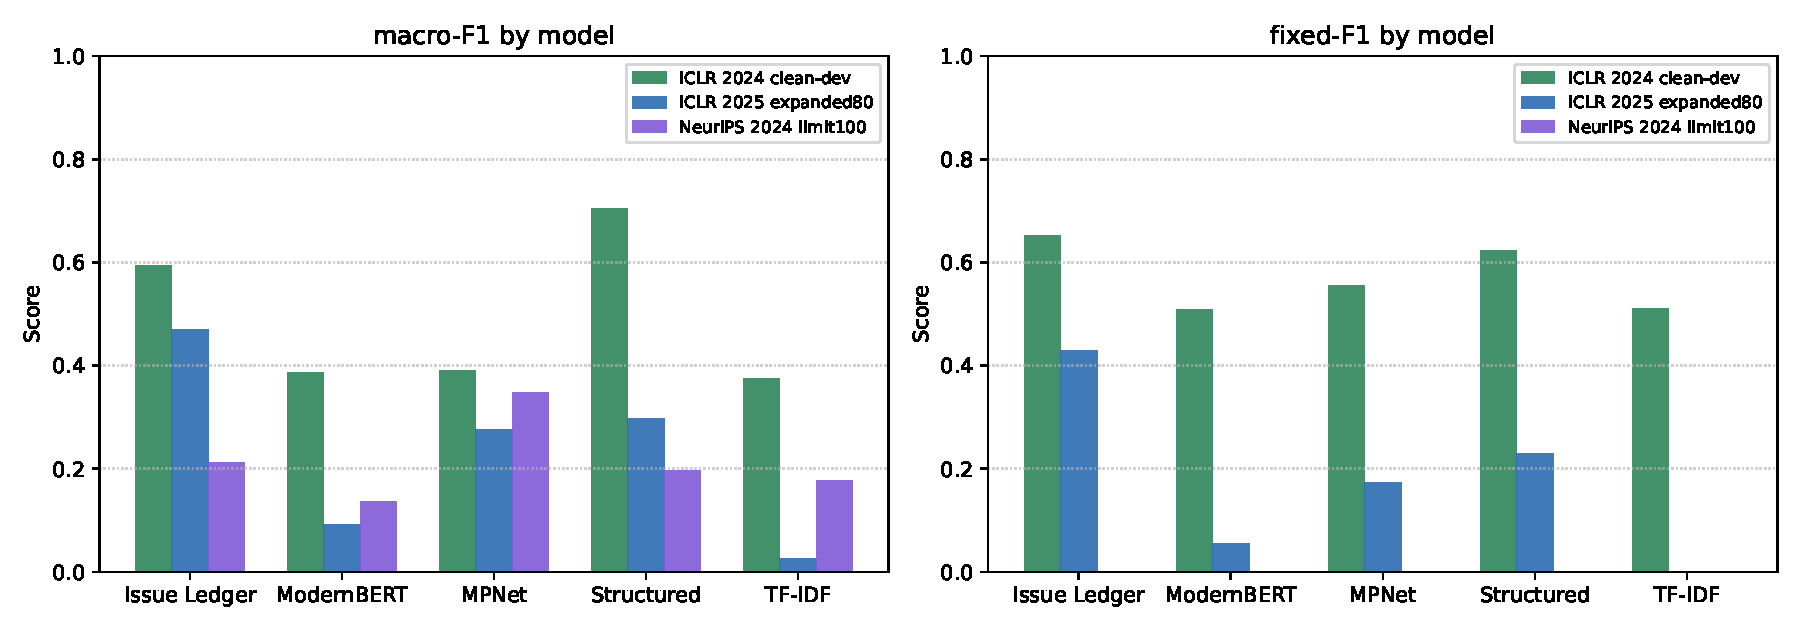
\includegraphics[width=\textwidth]{figures/figure2_transfer_breakdown.pdf}
\caption{Transfer-profile summary from three settings. Structured models and issue-ledger rules dominate in-domain and frontier settings on macro-F1, but fixed-label recovery remains weak under transfer and the NeurIPS 2024 frontier is dominated by unresolved cases.}
\label{fig:transfer-breakdown}
\end{figure*}

\subsection{RQ4: What Transfers Across Years and Venues?}

\begin{table}[t]
\centering
\scriptsize
\setlength{\tabcolsep}{3pt}
\begin{tabular}{p{0.28\linewidth}rrrr}
\toprule
Model & Accuracy & Macro-F1 & Fixed F1 & Regressed F1 \\
\midrule
TF-IDF & 0.050 & 0.026 & 0.000 & 0.000 \\
ModernBERT & 0.125 & 0.092 & 0.056 & 0.000 \\
MPNet & 0.312 & 0.276 & 0.174 & 0.500 \\
Structured & 0.150 & 0.298 & 0.229 & \textbf{0.800} \\
Issue ledger & \textbf{0.850} & \textbf{0.469} & \textbf{0.429} & 0.500 \\
\bottomrule
\end{tabular}
\caption{ICLR 2025 expanded80 standard-labeled active frontier. The frontier is intentionally hard and model-disagreement-heavy, so it supports transfer brittleness analysis rather than natural label-prevalence estimates.}
\label{tab:expanded80-transfer}
\end{table}

\begin{table}[t]
\centering
\scriptsize
\setlength{\tabcolsep}{2pt}
\begin{tabular}{p{0.25\linewidth}ccccc}
\toprule
Model & Acc. & Macro & Fixed & Partial & Unres. \\
\midrule
Issue Ledger & 0.500 & 0.211 & 0.000 & 0.167 & 0.679 \\
ModernBERT & 0.200 & 0.137 & 0.000 & 0.229 & 0.320 \\
MPNet & 0.550 & 0.348 & 0.000 & 0.516 & 0.875 \\
Structured & 0.362 & 0.197 & 0.000 & 0.545 & 0.244 \\
TF-IDF & 0.550 & 0.177 & 0.000 & 0.710 & 0.000 \\
\bottomrule
\end{tabular}
\caption{NeurIPS 2024 limit100 user-confirmed single-pass active frontier transfer from the ICLR 2024 model stack. No fixed or regressed examples are present in this frontier, so fixed/regressed F1 are unavailable for stronger interpretation.}
\label{tab:neurips100-transfer}
\end{table}


\textbf{In-domain to ICLR 2025} is still the strongest signal for proving in-year revision-aware gain, but both expanded80 and NeurIPS limit100 are purposefully hard.
Cross-venue transfer confirms the same pattern:
high aggregate scores alone can mask clinically important misses, while unresolved concerns remain the hardest safety-critical case.

The validated ICLR 2025 repro set is a stress test, not a full benchmark.
It reveals brittleness: the majority baseline and TF-IDF both reach 0.762 accuracy, while TF-IDF has fixed-label F1 of 0.000.
The expanded ICLR 2025 frontier removes the scale blocker at the active-frontier stage: it contains 322 candidates and 244 model-disagreement rows, and its 80-row validation packet has complete standard labels and evidence spans.
Table~\ref{tab:expanded80-transfer} shows this frontier remains difficult under transfer.
Table~\ref{tab:neurips100-transfer} shows the same trend in a different venue ecology and is included as a standard single-user cross-venue active frontier.
It also shows unresolved labels still dominating and fixed recovery absent in the current split.
Issue-ledger rules are strongest overall in this bounded frontier setting, while TF-IDF and encoder baselines have weak macro-F1 and poor fixed-case recovery.
This supports a cross-year brittleness claim, but not a broad prevalence claim, because the frontier is intentionally model-disagreement-heavy.
Because these frontiers are disagreement-harvested hard subsets, they should be read as stress-test transfer evidence rather than as a full distributional estimate of venue-wide revision behavior.
The ICLR 2023 random/stratified slice complements these frontiers with 80 standard rows and a fixed/partial/unresolved label mix of 5/49/26.
It supports bounded external-validity evidence by measured slice design, not a claim about natural venue prevalence.
Appendix Table~\ref{tab:cross-split-significance} reports stratified-bootstrap confidence intervals for all three standard splits; ranking uncertainty is small for the in-domain gap and substantially larger on transfer frontiers.

\subsection{RQ5: How Do Prompted LLM Baselines Behave Under Transfer?}

\begin{table}[t]
\centering
\scriptsize
\setlength{\tabcolsep}{2pt}
\begin{tabular}{p{0.28\linewidth}cccc}
\toprule
Model & ICLR24 & ICLR25 & NeurIPS & Mean \\
\midrule
Majority & 0.184 & 0.226 & 0.177 & 0.196 \\
GPT-5.5 (v2) & 0.350 & 0.081 & 0.171 & 0.201 \\
GPT-4.1 & 0.326 & 0.070 & 0.166 & 0.187 \\
GPT-4o-mini & 0.299 & 0.077 & 0.178 & 0.185 \\
GPT-4.1-nano & 0.210 & 0.161 & 0.126 & 0.166 \\
Qwen2.5-72B & 0.334 & 0.072 & 0.165 & 0.190 \\
GPT-4.1-mini & 0.347 & 0.066 & 0.181 & 0.198 \\
\midrule
Vote-3 (top) & 0.352 & 0.071 & 0.179 & 0.201 \\
Vote-3 (diverse) & 0.347 & 0.088 & 0.174 & 0.203 \\
Vote-3 (U-guard) & 0.345 & 0.092 & 0.170 & 0.202 \\
Vote-3 (U+F) & 0.350 & 0.094 & 0.167 & 0.204 \\
Vote-6 (all) & 0.344 & 0.064 & 0.177 & 0.195 \\
\bottomrule
\end{tabular}
\caption{Macro-F1 of prompted LLMs and vote ensembles on three standard-labeled splits. Voting improves in-domain stability but does not resolve cross-year brittleness on expanded80.}
\label{tab:prompted-llm-ensemble}
\end{table}


Table~\ref{tab:prompted-llm-ensemble} adds six prompted-LLM baselines, five vote-calibration variants, and a majority-label reference on the same standard-labeled splits.
In-domain ICLR 2024 is competitive for several prompted variants, but transfer remains brittle.
On ICLR 2025 expanded80, all prompted and ensemble variants remain below the majority-label macro-F1 baseline (0.226); the strongest calibrated vote reaches 0.094.
On NeurIPS limit100, the best prompted model reaches 0.181 macro-F1, while the best vote reaches 0.179 and stays near the majority baseline (0.177).
Model pooling therefore improves stability but does not close the longitudinal transfer gap.
Appendix Table~\ref{tab:prompted-llm-bootstrap} shows the same risk under bootstrap uncertainty: ICLR24 prompted rows are above majority, ICLR25 rows remain below majority, and NeurIPS24 rows mostly overlap the majority reference.
Appendix Table~\ref{tab:prompted-llm-significance} reports paired stratified-bootstrap significance against the majority baseline: prompted rows are reliably above majority in-domain, reliably below majority on ICLR25 expanded80, and statistically overlapping on NeurIPS24.

\begin{table*}[t]
\centering
\scriptsize
\setlength{\tabcolsep}{3pt}
\begin{tabular}{lrrrrrr}
\toprule
Variant & Prompt & Temp & Accuracy & Macro-F1 & U Recall & F Recall \\
\midrule
GPT-4o-mini & default & 0.0 & 0.062 & 0.077 & 0.015 & 0.250 \\
GPT-4o-mini & default & 0.3 & 0.038 & 0.020 & 0.015 & 0.000 \\
GPT-4o-mini & default & 0.7 & 0.038 & 0.021 & 0.015 & 0.000 \\
GPT-4o-mini & unresolved-strict & 0.0 & 0.062 & 0.032 & 0.015 & 0.000 \\
GPT-5.5(v2) & default & 0.0 & 0.088 & 0.081 & 0.045 & 0.250 \\
GPT-5.5(v2) & unresolved-strict & 0.0 & 0.100 & 0.059 & 0.091 & 0.000 \\
GPT-4.1-mini & default & 0.0 & 0.062 & 0.066 & 0.015 & 1.000 \\
GPT-4.1-mini & unresolved-strict & 0.0 & 0.100 & 0.086 & 0.061 & 1.000 \\
GPT-4.1-nano & default & 0.0 & 0.350 & 0.161 & 0.379 & 0.750 \\
GPT-4.1-nano & unresolved-strict & 0.0 & 0.412 & 0.171 & 0.485 & 0.250 \\
\bottomrule
\end{tabular}
\caption{Expanded80 decoding/prompt ablation for prompted transfer. Temperature increases are uniformly harmful. Unresolved-strict prompting is model-dependent: it hurts GPT-4o-mini and GPT-5.5(v2) macro-F1, while improving GPT-4.1-mini and GPT-4.1-nano unresolved recall and macro-F1 with trade-offs on fixed recall.}
\label{tab:prompted-llm-temp}
\end{table*}


Table~\ref{tab:prompted-llm-temp} shows targeted decoding/prompt ablations on expanded80.
Raising temperature (0.0 to 0.3/0.7) lowers macro-F1 from 0.077 to around 0.020, so transfer errors are not resolved by sampling diversity.
Unresolved-strict prompting is model-dependent: it hurts GPT-4o-mini and GPT-5.5(v2), but improves GPT-4.1-mini and GPT-4.1-nano with different fixed-recall trade-offs.
Even with those gains, absolute transfer performance remains low and below the majority baseline.
Full offline calibration-rule search results are reported in Appendix Table~\ref{tab:prompted-llm-postprocess-rules}.

\begin{figure*}[t]
\centering
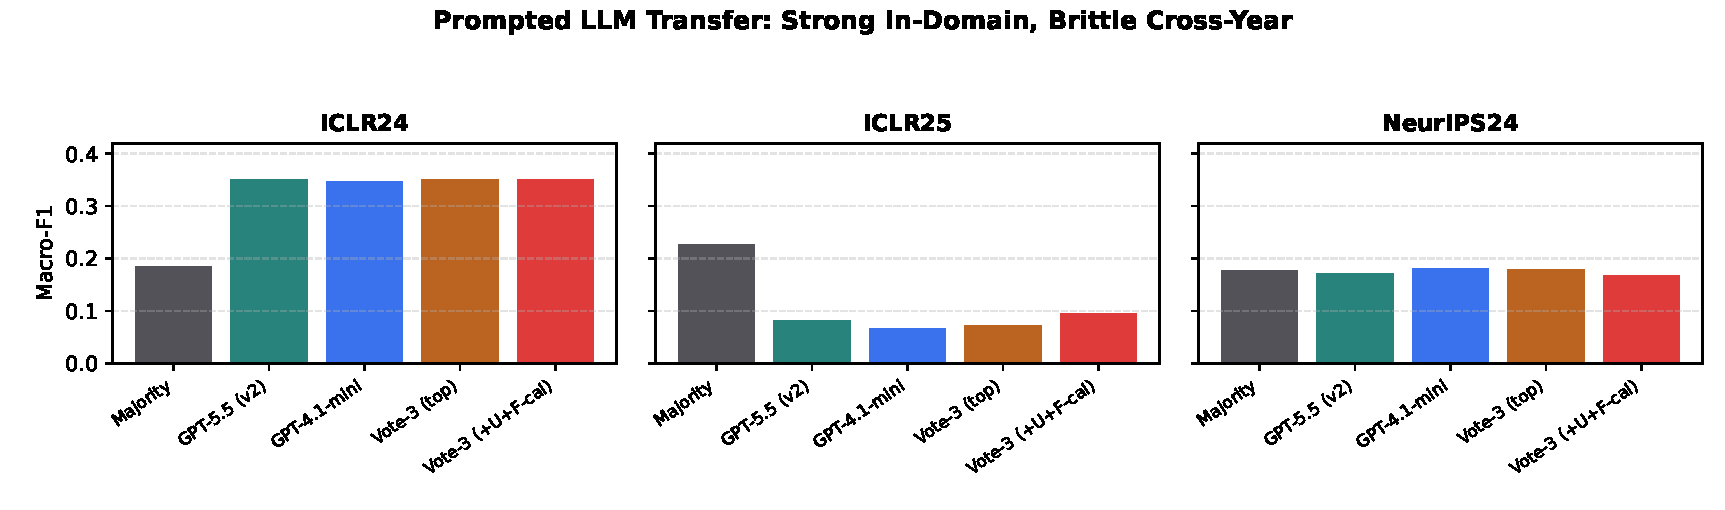
\includegraphics[width=\textwidth]{figures/figure3_prompted_llm_transfer.pdf}
\caption{Prompted-LLM transfer profile with majority baseline and vote ensembles, including calibrated unresolved/fixed safeguards. Ensemble voting improves ICLR 2024 stability but does not recover cross-year robustness on expanded80.}
\label{fig:prompted-llm-transfer}
\end{figure*}

\begin{figure*}[t]
\centering
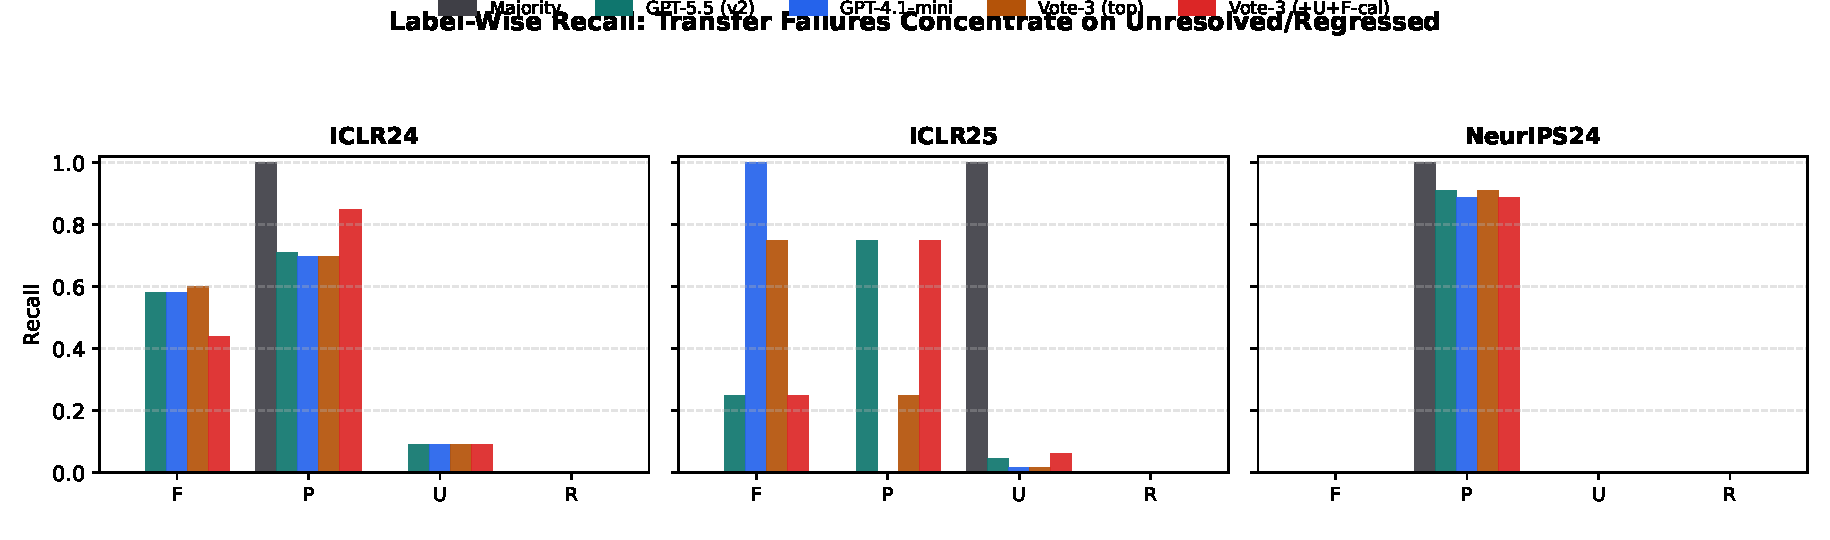
\includegraphics[width=\textwidth]{figures/figure4_prompted_llm_label_recall.pdf}
\caption{Label-wise recall for majority baseline, prompted LLMs, and vote ensemble. Cross-year failures are dominated by unresolved under-recovery and zero regressed recall under prompted transfer.}
\label{fig:prompted-llm-recall}
\end{figure*}

\begin{figure*}[t]
\centering
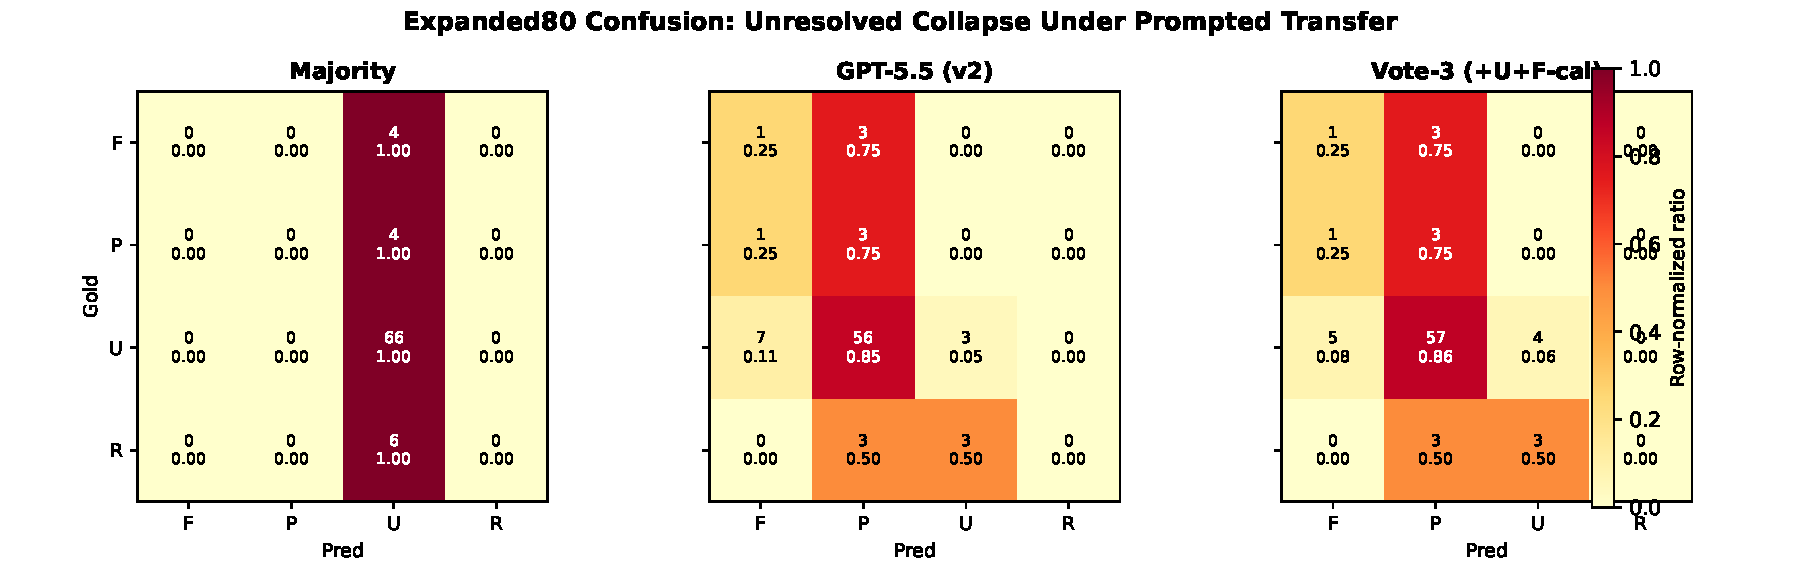
\includegraphics[width=\textwidth]{figures/figure5_expanded80_confusion.pdf}
\caption{Expanded80 row-normalized confusion matrices for majority baseline, GPT-5.5(v2), and Vote-3(+U+F-cal). Prompted transfer over-credits unresolved concerns as fixed/partial, while calibrated safeguards increase unresolved recovery but introduce additional tradeoffs.}
\label{fig:prompted-llm-confusion}
\end{figure*}

Figure~\ref{fig:prompted-llm-recall} explains why pooled prompted systems still fail under transfer.
In ICLR 2025 expanded80, prompted systems frequently over-credit unresolved cases as fixed or partial, so unresolved recall collapses to near-zero levels while regressed recall remains zero.
In NeurIPS limit100, the user-confirmed active frontier contains only partially-fixed and unresolved labels, and prompted models again collapse unresolved recall to zero by over-predicting partially-fixed.
Figure~\ref{fig:prompted-llm-confusion} localizes this failure in confusion space: most unresolved rows are reassigned to fixed/partial columns under prompted transfer.

\begin{figure*}[t]
\centering
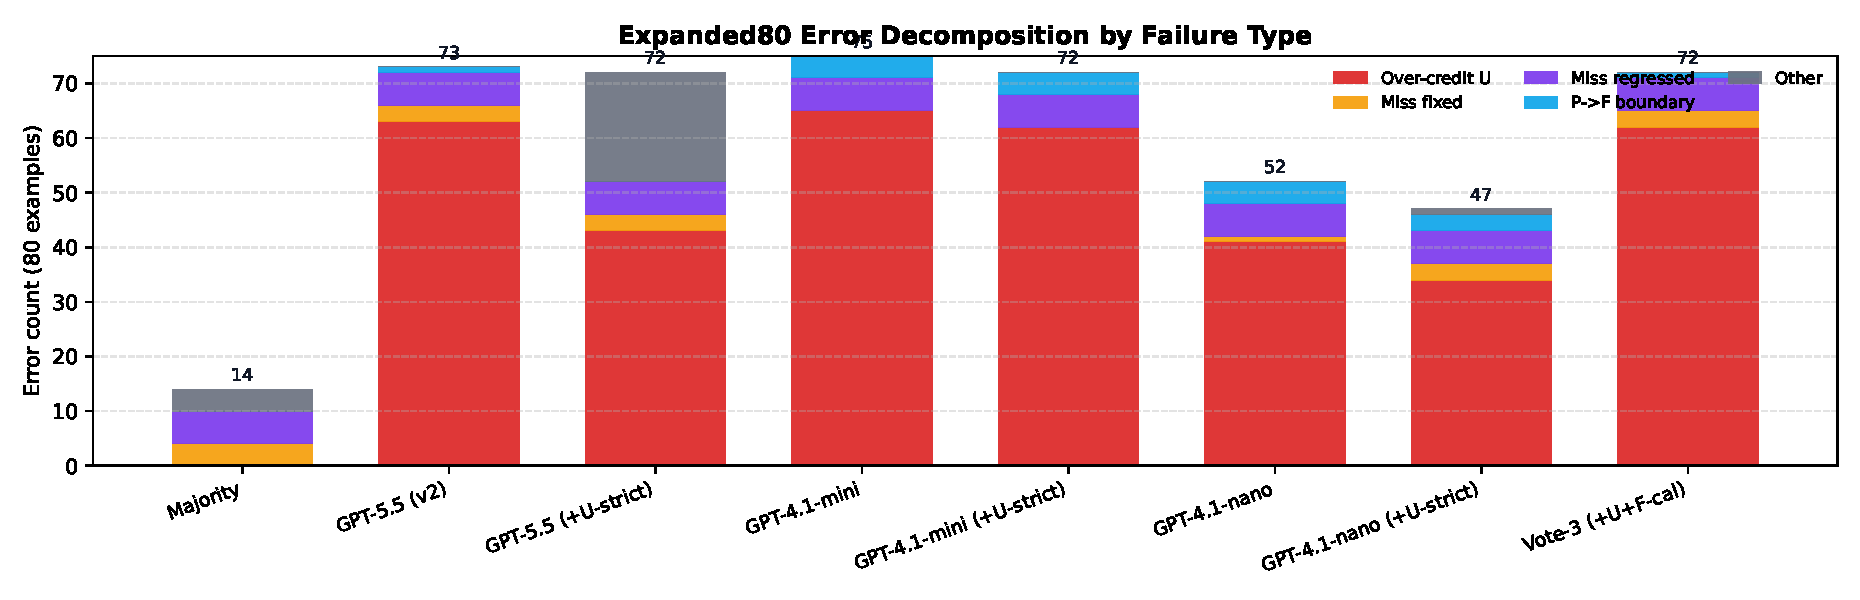
\includegraphics[width=\textwidth]{figures/figure6_expanded80_error_stack.pdf}
\caption{Expanded80 stacked error decomposition. Over-crediting unresolved concerns dominates all prompted variants; unresolved-strict prompting reduces this category for GPT-5.5, GPT-4.1-mini, and GPT-4.1-nano, but transfer brittleness remains.}
\label{fig:prompted-llm-error-stack}
\end{figure*}

Figure~\ref{fig:prompted-llm-error-stack} quantifies the same pattern at error-type granularity.
Across models, over-crediting unresolved concerns is the largest error bucket by a wide margin, while regression misses remain persistent.
These label-level failures explain why aggregate in-domain gains do not translate into robust transfer behavior.
